% \documentclass[sigconf, screen, review]{acmart}
\documentclass[sigconf, nonacm]{acmart}
\usepackage{colortbl}
\usepackage{dblfloatfix}
\usepackage{placeins}

%% \BibTeX command to typeset BibTeX logo in the docs
\AtBeginDocument{%
  \providecommand\BibTeX{{%
    Bib\TeX}}}

%% end of the preamble, start of the body of the document source.
\begin{document}

\title{Torchlight: Diffusion-based Network Trace Generation from the DARPA Searchlight Dataset}

% \author{Ray Zhao}
% \affiliation{%
%  \institution{University of Southern California}
%  \city{Los Angeles}
%  \state{California}
%  \country{}}
% \email{rdzhao@usc.edu}

% \author{Alefiya Hussain}
% \affiliation{%
%   \institution{USC/ISI}
%   \city{Los Angeles}
%   \country{}}
% \email{hussain@isi.edu}

\renewcommand{\shortauthors}{Zhao, Hussain}

\begin{abstract}
  At present, there is a severe lack of both comprehensive and realistic labeled datasets
  for machine learning applications in the networking domain. Predominantly, prior generative
  work has focused on lower-dimensional representations that rely on aggregating flow 
  characteristics and lack the fine-grain of raw network traces. This results in suboptimal
  performance in machine learning contexts and limited applications outside of those 
  contexts. This has induced a push for new generative techniques to provide 
  synthetic data for usage both on its own and layered in with real data as augmentation.
  In this paper, we present Torchlight, a diffusion-based
  generation framework built atop and extending techniques first introduced in 
  \textit{NetDiffusion} \cite{jiang2024netdiffusion} using DARPA Searchlight 
  \cite{ardi2022} data to generate synthetic network traces
  for video streaming applications. We demonstrate the efficacy of Torchlight in generating
  synthetic network traces that reasonably resemble real-world data and perform notably well
  in classification tasks. 
\end{abstract}

\maketitle

\section{Introduction}
There's a large need and general scarcity of labeled network datasets,
as high-quality data is often expensive and frought with privacy concerns,
and the datasets that do exist are often left rarely update over time.
Synthetic data generation techniques aim to solve this problem, but prior
GAN based methodologies have been limited in their ability to generate
raw, high-dimensional traces and often rely on aggregating flow characteristics,
which results in data that lacks statistical fidelity to real data and performs
much more poorly in machine learning tasks. The highly specific formatting of
these types of condensed traces also renders them generally incompatible with
traditional tools like Wireshark and tcpdump.

In recent years, the advent of diffusion models have solved many of the
problems that plague older GAN frameworks, being able to capture much
more complex patterns and relationships. They also usually offer much more
stability in the training process, in which GANs are notably finnicky.
Additionally, their now near-hegemony in the image generation space has
enabled a wide base of development support in the diffusion community 
and has also made available many "plug and play"
means of constraining generation to appropriate enough scopes for specific generation
tasks like the one at hand.

As it pertains to Torchlight, we build on the NetDiffusion framework pioneered
by Jiang et al. \cite{jiang2024netdiffusion} to generate synthetic network traces for video
streaming applications, using the DARPA Searchlight dataset \cite{ardi2022} as
our base. Our contributions are as follows:

\begin{enumerate}
  \item \textbf{Successful application of NetDiffusion techniques on the Searchlight Dataset}:
  Using the pre-processing and post-processing code provided by Jiang et al., we were able to
  successfully generate synthetic traces that performed capably on its own as training
  data for classification tasks as well as when used in conjunction with real data 
  as augmentation.
  \item \textbf{Streamlining the generation process}: While the original NetDiffusion codebase
  used exterrnally-built WebUIs for LoRA fine-tuning as well as the Controlnet, 
  these two major components were integrated into the codebase such that the 
  entire process can be run from a single script.
\end{enumerate}

\section{Motivation \& Related Work}
Publicly available network data is crucial in this field for enabling continued
researhc and development of new networking technologies and techniques. While useful for
more traditional networking analysis tasks, machine learning applications have been driving
much of the development in use-cases like anomaly detection and traffic classification and 
in particular have largely relied on these datasets.

\subsection{Cost and Scarcity}
Notable datasets like DARPA Searchlight and CAIDA have been essential 
in the development of new networking technologies, but expensive and complex
to develop and then maintain. Entities with the means to develop these datasets
often have little incentive to release them to the public, as they are often
highly proprietary and run into ethics concerns. Even when they are released, 
they are often left to stagnate and lose relevance over time, as the networking
landscape is highly dynamic.

\subsection{Data Augmentation}
In the absence of high-quality labeled data, data augmentation has been a popular
technique, especially in computer vision, to extend the utility of exisiting
and the models with which they are used. Synthetic data generation has been
successful across domains, with GANs being dominant in the image generation space
and autoencoders being popular in creating synthetic text data. 

The most notable application of synthetic data generation in networking has been
in the realm of flow-based data, where the data is aggregated into flows and then
used to generate synthetic data. This has been successful in some applications, 
most notably NetShare \cite{netshare-sigcomm2022}, which produces NetFlow-like aggregates 
on network traffic. The limited dimensionality of these aggregates, however, 
means much coaser-grained pattern capture and limited utility outside of 
pure model training.

The original authors of NetDiffusion \cite{jiang2024netdiffusion} have shown that
NetFlow data performs poorly in classification tasks in comparison to raw 
traffic data, and as such have been motivated to develop a new framework
that can generate raw traces.

\section{Methods}
Here we outline the framework used in Torchlight to generate synthetic network traces,
which is built atop NetDiffusion \cite{jiang2024netdiffusion} and updates and streamlines it.
Our approach is segmented into five primary moving parts:

\begin{enumerate}
  \item Conversion of raw network traces in \verb|.pcap| format into images
  \item Fine-tuning a pretrained diffusion model with LoRA on the labelled images
  \item ControlNet constrained generation of synthetic traces
  \item Color correction and network compliance post-processing
  \item Conversion of generated and processed images back into \verb|.pcap| format
\end{enumerate}

\subsection{Trace to Image Conversion}
This work is anchored on the core concept of encapsulating raw network data
into a dense image format. Pixels in images inherently form high-dimensional 
patterns and structures with long-range, highly non-linear dependencies.
While tabular formats typically engender points as indepedent entities, images 
much more adeptly preserve temporal and spatial relationships between network
flows that traditional tabular formats do not. Development in the image space has always been
rapid and deep-learning and subsequent generative techniques have been refined 
over time to capture these complex relationships. As importantly, this format
allows us to exploit the maturity and computational throughput
of image-based deep learning. Diffusion models are
the newest and most powerful of these techniques, and have been shown to be of
great utility in the image generation space. We will delve into more detail on
this in the next section.

Our image representation is expressed with the nPrint \cite{holland2022towards} format, which
standardizes the irregular and high-dimensional network patterns of raw 
traces into a consistent bit-mapped format, where the presence or absence of a bit
in the packet header is denoted 1 or 0 respectively, and a missing header bit is
represented as -1. The payload content is not encoded since it's often encrypted, 
but size of payloads can be inferred from other encoded header fields. 
With this, a sequence of pcaps is converted into a matrix which can be formatted
as an image. A set bit (1), an unset bit (0), and a vacant bit (-1) are 
represented by green, red, and blue respectively. 
Due to the limitations in generative models’ capability to handle very high
dimensional data and standard image processing practice, we group packets in 
groups of 1024, resulting in a $1088 \times 1024$ image with each row of pixels
representing a packet in the network traffic flow as shown in Figure 2. 

\subsection{Model Fine-Tuning}
\subsubsection{Why diffusion models?}
Diffusion models fundamentally operate on the principle of iteratively updating
a set of latent variables to approximate a true data distribution, taking
a randomly initialized amount of noise and progressively refining it to
generate an image. A differential equation is used to control the transformation
of an initial noise vector $\mathbf{z}$ into a data point $\mathbf{x}$ over a 
series of time steps. This process is modeled by estimating the gradient of the
log-likelihood of the data with respect to the noise vector, and then using this
gradient to update the noise vector. Diffusion models typically operate in the
context of "text-to-image" synthesis, where a text prompt guides the 
generation of an image by conditioning the noise vector on the text. This
conditioning steers the data distribution from a general uniform prior distribution
to a more specific one fitted to the text prompt.

This process lends a number of advantages to diffusion, as opposed to other
generative techniques. Diffusion models have been shown to be adept at capturing
highly complex and intricate relationships and generating high-resolution
images. The text conditioning also allows for a high degree of control over
the generated images, as the text can be used to guide the generation process
in a way that is not possible with other generative models. Lastly,
diffusion models are highly stable and easy to train, as they do not require
the adversarial training that GANs do, and are much less prone to mode collapse.
Their stable gradient dynamics and ability to be seeded in training
ensures not just consistent but reproducible training results.

\subsubsection{Fine-tuning with LoRA.} Training a diffusion model from scratch
is highly computationally intensive and expensive, especially considering that
existing models are often trained on billions of images. While good for general
applications, base models like Stable Diffusion are too broad for our purposes. 
While a text prompt like "pixelated network data: dash, 1080" is what we end up 
using in our end-stage model, the base model would produce something 
like a pixelated image of a dash, which is not useful for our purposes. Low-Rank
Adaptation (LoRA) is a technique that allows us to fine-tune a pre-trained model
on a smaller dataset, which is much more computationally feasible. LoRA works by
attaching a low-rank matrix to the model's parameters and then training just 
the low-rank matrix on a new dataset. This allows us to adapt the stylistic and
color characteristics of the model to our specific dataset without having to
retrain the entire model.

In the fine-tuning process, we attach to every image a caption that corresponds
to the various characteristics of the image. For example, the image for
a network flow using the Wireguard VPN streaming 1080p video using DASH over
HTTP3 would be captioned "pixelated network data: wireguardptp, dash, 1080 hhtp3".
Hundreds of such image-caption pairs are then used to fine-tune the model over
the course of thousands of epochs to adapt the model to the specific 
color and stylistic characteristics of the images used to fine-tune it. 
The choice of caption is crucial and achieves two main objectives:
it gives the model a specific vocabulary that reduces ambiguity and minimizes
interference from the original word embeddings of the base model.

\subsection{Constrained Generation}
Even though fine-tuning can result in very high-quality output, it can
be very abstract and deviate greatly from the stricter bounds of network 
traffic data. To constrain the output, we can employ a ControlNet, which
is a separate neural network that sits atop the diffusion model and
modifies the output to be rigidly within the bounds defined by the 
ControlNet. Generally, a ControlNet is trained on a specific type of
spatial constraint, like poses, depth mapping, masks, or in our case,
canny edge detection. In the case of canny edge detection, the ControlNet 
takes as input a text prompt and the canny edges extracted from a sample image
to use as "guardrails" to guide the diffusion model in generating the final image.
ControlNet enables us to generate images that are not just high-quality,
but also highly compliant with the structure of network traffic.

\subsection{Post-Processing}
While the constrained diffusion model generates high-fidelity images
that greatly \textit{resemble} network traffic, use outside of ML tasks
require that the flows these images represent comply with network standards 
and the multitudes of inter and intra packet dependices that enable use 
in traditional networking applications. While ControlNet can do a lot to
ensure resemblance, it cannot guarantee compliance. To this end, 
we must apply a series
of post-processing steps to the generated images to ensure that they are
compliant with network standards. Broadly, these rules can be put into two
categories:
\begin{enumerate}
  \item \textbf{Inter-Packet}: Rules that govern the sequencing between
  header fields between packets in a flow, like the SYN / SYN-ACK handshake
  that initiates a TCP connection, the incorrect alignment of which can
  cause the connection to fail.
  \item \textbf{Intra-Packet}: Rules that organize the structure of individual
  packets, like the ordering of header fields within a packet and checksums
  that ensure the integrity of the packet.
\end{enumerate}

Most of the work of creating a systematic approach that comprehensively 
identifes and corrects these errors has been done by original 
NetDiffusion authors, and we have largely built on their work in this
area. The post-processing steps are fully automated and accomplished
by traversing two intra-packet and inter-packet dependency trees built
with domain knowledge. A notable challenge the authors faced was
time-stamp assignment for packets, which was resolved by sampling 
original timestamps from real data to produce similar timestamp distributions
in the synthetic data. This post-processing ensures that the generated
traffic can be smoothly converted into raw network formats and utilized
in non-ML contexts.

\subsection{Image to Trace Conversion}
The final step in the process is to convert the generated images back
into network traces and is relatively straightfoward.
This is done by reversing the process used to convert
the original traces into images. The generated images are first converted
into nPrint format, and then the nPrint format is converted back into
a sequence of pcaps. The post-processing steps ensure that the generated
pcaps are compliant with network standards and can be used in traditional
networking applications.

\section{Evaluation}
The assessment of this framework is done primarily in 2 ways: assessing
the statistical differences between the original and synthesized data and
gauging its performance
in machine learning classification tasks. While the original NetDiffusion paper
goes into great detail about the performance of the generated in outside
applications, we focus on a statistical analysis and classification performance,
arugably the most common use-case for synthetic data in networking.

\subsection{Dataset Overview \& Generation}
The data used is the DARPA Searchlight dataset \cite{ardi2022}, which is a large
collection of network traces from a variety of sources and applications. Searchlight
was collected over a period of 6 months and contains a wide variety of traffic types,
including video streaming, web browsing, and file transfers all coordinated on a 
complex testbed that includes a variety of network devices and topologies, making it
highly representative of real-world network traffic. 

We focus on video streaming
using tiered topology traffic in our work. All data is routed through a VPN, configured
in either \textit{site-to-site} (STS) or \textit{point-to-point} (PTP) 
configuration, and a variety of video resolutions and streaming and transport
protocols were used, all of which are shown in Table 1. In lieu of "micro-level" 
and "macro-level" service distinctions as made in the original NetDiffusion paper, 
we use these different labels to evaluate statistical differences and
classification performance 

There are 342 video experiments using tiered topology to record video traffic. 10
images were synthesized with the canny edges from each "parent" image, resulting in 
3420 total synthetic samples.

\begin{table}[h!]
    \centering
    \begin{tabular}{@{}ll@{}}
      \midrule
    \textbf{Category} & \textbf{Classes} \\ \midrule
    \textbf{Encryption (VPN)} & {IpsecPTP, WireguardPTP, WireguardSTS} \\
    \textbf{Resolution} & 576p, 720p, 1080p \\
    \textbf{Streaming Protocol} & DASH, HLS, HTML5 \\
    \textbf{Transport Protocol} & HTTP/1.1, HTTP/1.1+TLS, HTTP/2, HTTP/3  \\
    \bottomrule
    \end{tabular}
    \caption{Relevant Categories and their Classes}
    \label{tab:config_features}
\end{table}

\subsection{Statistical Analysis}
The core premise of generating synthetic data is to try to achieve a robust
statistical resemblance to the original data. The statistical measure we opt 
for is Jensen-Shannon distance (JSD), which is a symmetric and finite measure of
the similarity between two probability distributions. The JSD between two distributions
is calculated by first computing the KL divergence between the two distributions and 
taking the average. The JSD is bounded between 0 and 1, with
0 indicating that the two distributions are identical and 1 indicating that the
two distributions are completely different. In our case, we take the JSD between each
synthetic example and its "parent" image that provided edges to the ControlNet.

\begin{figure*}[htbp]
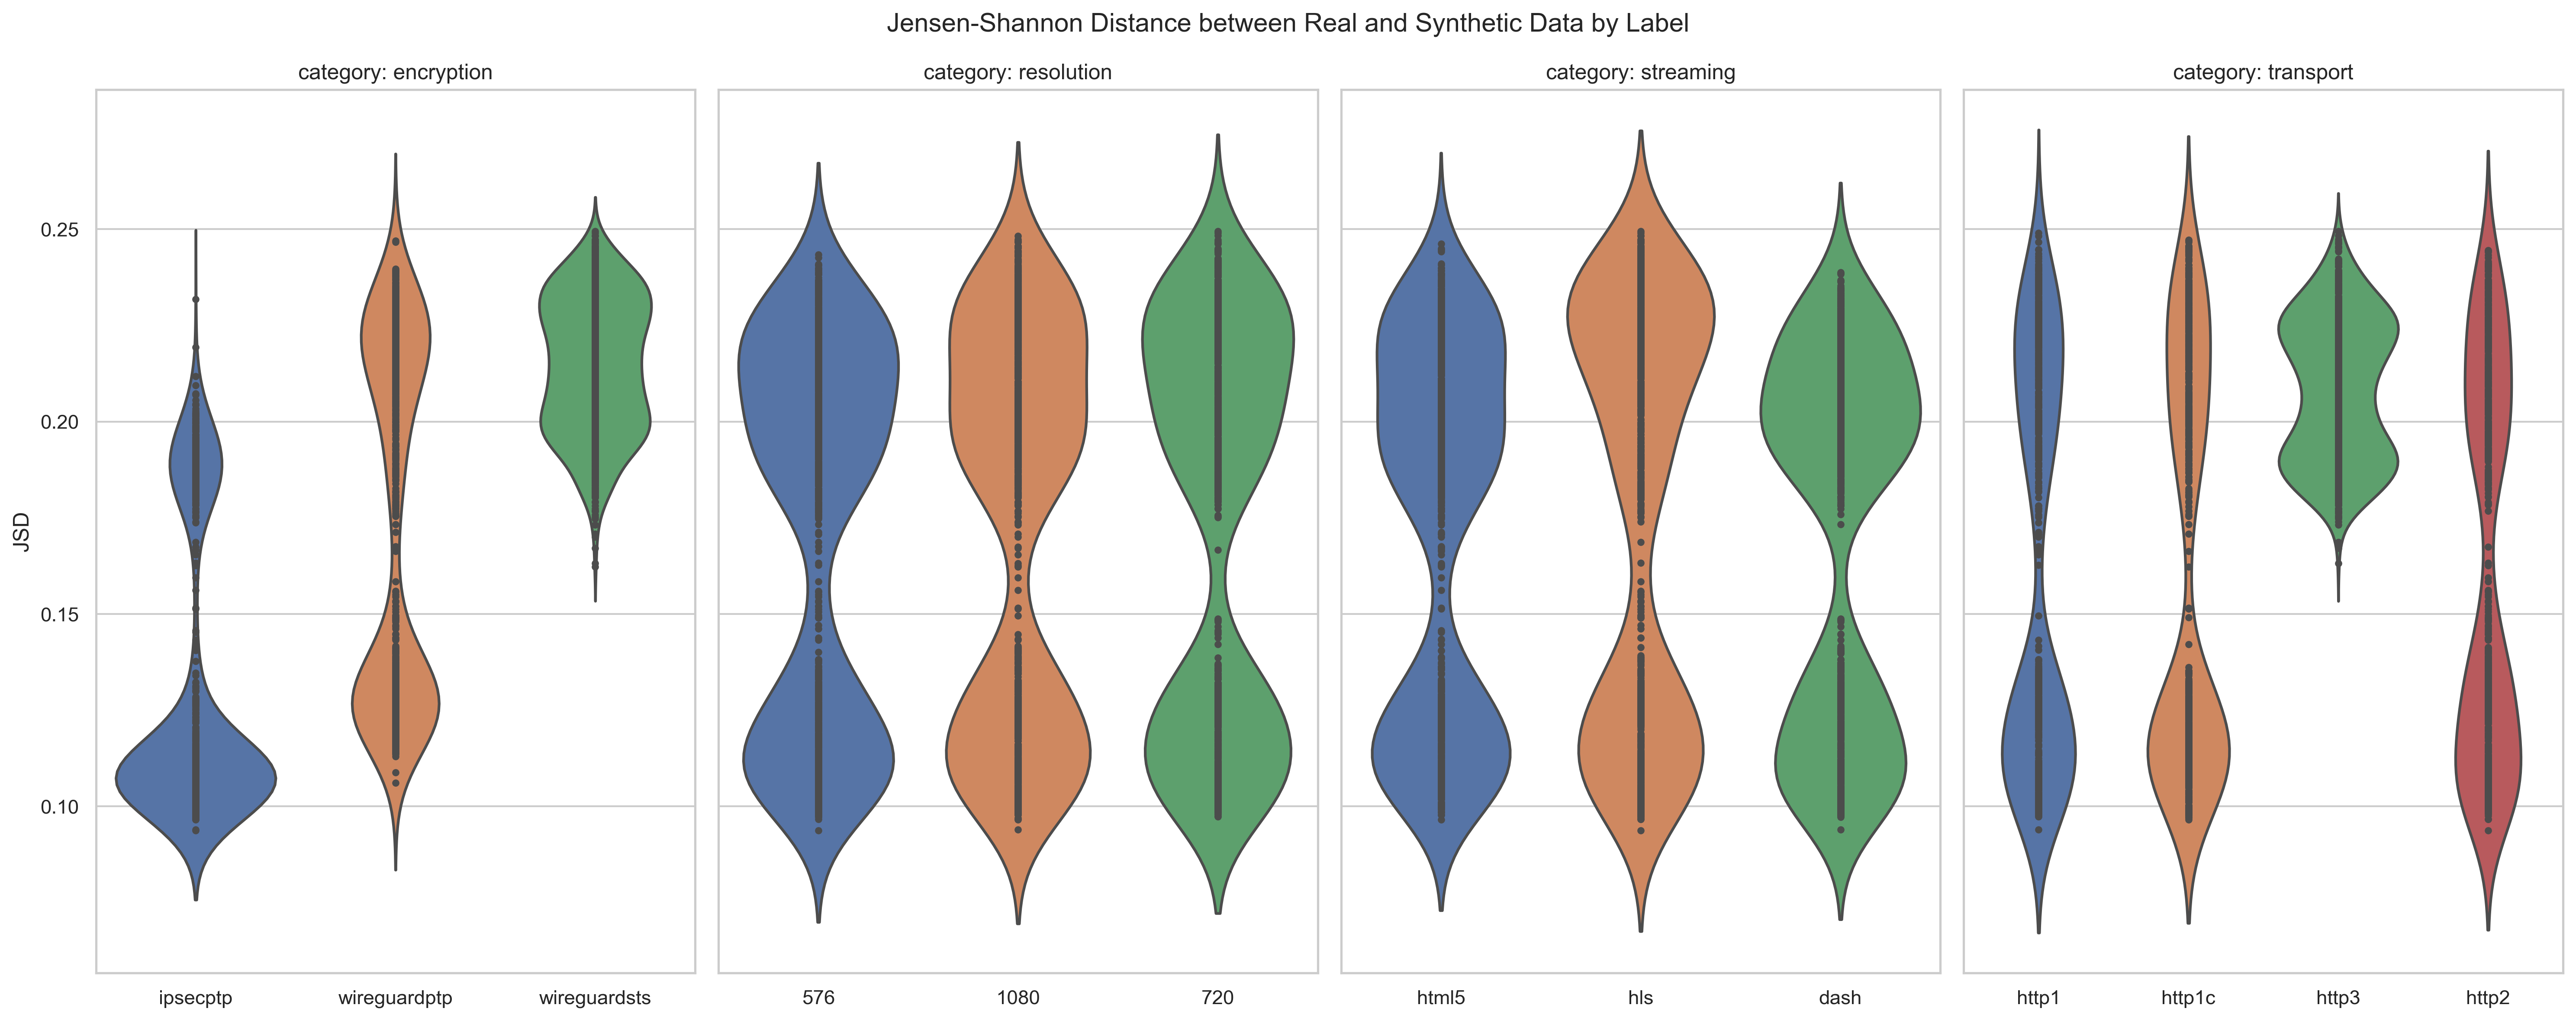
\includegraphics[width=1\textwidth]{../src/evaluation/figures/jsd_violin.png}
\caption{Jensen-Shannon Distance Between Real and Generated Data}
\label{fig:jsd_violin}
\end{figure*}
\FloatBarrier

Interestingly enough, the deviations tend to be bimodal, with large amounts
centered around 0.10 or around 0.20. The syntheitc data seems to generally capture
resolution and streaming information relatively uniformly while for encryption and transport
it seems to perform markedly better on some classes and worse on others.

\subsection{Classification Results}
For classification tasks, we use three main models: decision trees, random forests,
support vector machines. Accuracy is the metric used, as classes are exactly balanced
and accuracy is a good measure of overall performance. A model is trained for every 
category, performing multi-class classification at each instance. We tested performance
in four distinct scenarios:

\begin{enumerate}
  \item \textbf{Train on real data, test on real data}:
  Using 5-fold cross validation done over 10 runs, 
  evaluate multi-class performance on all three models on every category, giving
  a clear baseline as to how well the models can perform on the original data.
  \item \textbf{Train on synthetic data, test on real data}: Using traditional 
  train-test splitting at a 4:1 ratio,
  done over 100 runs, we train each model using only synthetic data and test on real
  data, maintaining the size (342) to ensure a fair comparison
  \item \textbf{Train on real data, test on synthetic data}: Using traditional 
  train-test splitting at a 4:1 ratio, done over 100 runs, we train each model using real
  data and test on synthetic data, maintaining the size (342) to ensure a fair comparison.
  \item \textbf{Mixed data proporrtions}: Using traditional train-test splitting at a 4:1 ratio
  done over 100 runs, after splitting, we replace some proportion $p$ of the training
  data with synthetic data, where $p \in \{0.1, \ldots, 0.9\}$ and test on all real 
  data with random forests to evaluate performance in a data augmentation scenario.
\end{enumerate}

\subsubsection{Results on no \& complete synthetic data usage}: The results presented
in Table 2 illustrate that our data performs reasonably well in classification tasks. 
The drop in performance when using synthetic data is expected, as the synthetic data
is not perfect and will not capture all the intricacies of the real data. The drop
in performance is most pronounced in the encryption and transport categories, which
is likely due to the complexity of these categories and the difficulty in capturing
the nuances of these categories in the synthetic data. The performance of the models
doesn't deviate as much for resolution and streaming, which the real/real models don't
perform as well on in their own right. Lastly an interesting comparison is the
performance of the models trained on real data and tested on synthetic data, which
actually relatively closely to the performance of the models trained on synthetic data,
which shows that the synthetic data is still able to capture a robust amount of 
the patterns inherent in the real data.

% \begin{table}[h!]
%   \centering
%   \begin{tabular}{lllll}
%   \toprule
%   \textbf{category} & \textbf{real/real} & \textbf{synthetic/real} & \textbf{real/synthetic} \\ \midrule
%   \multirow{encryption}   & 1.00 & 0.615 & 0.555 \\
%   \multirow{resolution} & 0.361 & 0.336 & 0.385 \\
%   \multirow{streaming} & 0.345 & 0.345 & 0.342 \\
%   \multirow{transport} & 0.803 & 0.296 & 0.302 \\
%   \bottomrule \\
%   \end{tabular}
%   \caption{The best performance of different models on various training and testing scenarios}
%   \end{table}

\begin{table}[h!]
\centering
\begin{tabular}{lllll}
\toprule
\textbf{category} & \textbf{real/real} & \textbf{synthetic/real} & \textbf{real/synthetic} \\ \midrule
encryption   & 1.00 & 0.615 & 0.555 \\
resolution & 0.361 & 0.336 & 0.385 \\
streaming & 0.345 & 0.345 & 0.342 \\
transport & 0.803 & 0.296 & 0.302 \\
\bottomrule \\
\end{tabular}
\caption{The best performance of different models on various training and testing scenarios}
\end{table}


\subsubsection{Results on mixed data}: Presented in Figure 2 is the performance of 
the random forest model as the mixing rate goes from 0 to 1, and observable is the 
progression of performance. Notably encryption stays relatively stable until all of 
the data is replaced and streaming protocol actually improves with a small amount
of synthetic data and then falls off quickly as more real data is replaced. 
Resolution reamins relatively stable all throughout and streaming actually 
improves near monotonically with the addition of synthetic data. This
also provides an extension to the performance comparisons in Table 2, 
showing that the synthetic data can be used effectively as an augmentation
tool.

\begin{figure}[h!]
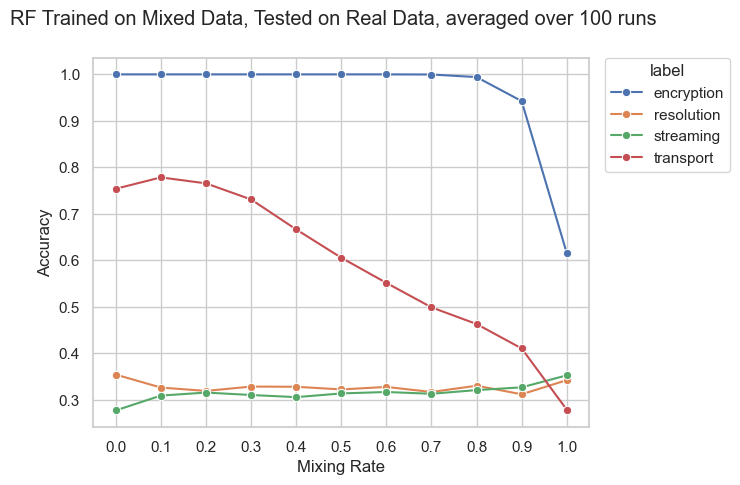
\includegraphics[width=0.5\textwidth]{../src/evaluation/figures/mixing.png}
\caption{Performance of RF on Mixed Data Proportions}
\label{fig:data_mixing}
\end{figure}
\FloatBarrier

\subsubsection{Feature Comparisons}
Another useful way to observe the fidelity of the synthetic data is to compare
the feature importance of the models trained on real and synthetic data.
Using random forests and training over 100 runs, we take the 10 most important
features of each run and collect the 10 most commonly occuring features.
We see that there's at least some overlap in the features that are most important
to the models, which is a good sign that the synthetic data is capturing 
important patterns in the real data.

\begin{table*}[h!]
\centering
\begin{tabular}{|c|c|c|c|c|}
\hline
\textbf{rank} & \multicolumn{2}{c|}{\textbf{encryption type}} & \multicolumn{2}{c|}{\textbf{resolution}} \\ \hline
& \textbf{real / real} & \textbf{synthetic / real} & \textbf{real / real} & \textbf{synthetic / real} \\ \hline
1 & udp\_sport\_4 & \cellcolor[HTML]{02B021}ipv4\_tl\_13 & ipv4\_ttl\_3 & \cellcolor[HTML]{02B021}ipv4\_cksum\_15 \\ \hline
2 & udp\_dport\_1 & \cellcolor[HTML]{02B021}ipv4\_tl\_15 & ipv4\_tl\_11 & udp\_dport\_5 \\ \hline
3 & ipv4\_hl\_3 & \cellcolor[HTML]{02B021}ipv4\_tl\_14 & udp\_len\_13 & tcp\_opt\_83 \\ \hline
4 & ipv4\_foff\_12 & ipv4\_id\_0 & udp\_cksum\_14 & tcp\_opt\_35 \\ \hline
5 & ipv4\_tl\_5 & \cellcolor[HTML]{02B021}ipv4\_tl\_11 & ipv4\_cksum\_15 & tcp\_opt\_82 \\ \hline
6 & udp\_dport\_4 & \cellcolor[HTML]{02B021}ipv4\_tl\_9 & ipv4\_id\_7 & tcp\_dprt\_4 \\ \hline
7 & ipv4\_tos\_6 & \cellcolor[HTML]{02B021}ipv4\_tl\_12 & tcp\_seq\_10 & tcp\_sprt\_2 \\ \hline
8 & ipv4\_tl\_13 & \cellcolor[HTML]{02B021}ipv4\_tl\_10 & ipv4\_cksum\_10 & tcp\_dprt\_5 \\ \hline
9 & ipv4\_proto\_5 & \cellcolor[HTML]{02B021}ipv4\_tl\_8 & tcp\_wsize\_12 & tcp\_sprt\_7 \\ \hline
10 & ipv4\_tl\_10 & tcp\_ackn\_8 & ipv4\_tl\_5 & \cellcolor[HTML]{02B021}ipv4\_cksum\_0 \\ \hline
\end{tabular}
\begin{tabular}{|c|c|c|c|c|}
\hline
\textbf{rank} & \multicolumn{2}{c|}{\textbf{streaming}} & \multicolumn{2}{c|}{\textbf{transport}} \\ \hline
& \textbf{real / real} & \textbf{synthetic / real} & \textbf{real / real} & \textbf{synthetic / real} \\ \hline
1 & udp\_len\_5 & \cellcolor[HTML]{02B021}ipv4\_cksum\_15 & udp\_len\_12 & \cellcolor[HTML]{02B021}ipv4\_tl\_2 \\ \hline
2 & ipv4\_tl\_13 & \cellcolor[HTML]{02B021}ipv4\_tl\_1 & ipv4\_tl\_9 & ipv6\_hl\_4 \\ \hline
3 & ipv4\_id\_13 & udp\_dport\_7 & tcp\_sprt\_15 & ipv4\_opt\_245 \\ \hline
4 & udp\_cksum\_0 & udp\_dport\_3 & udp\_sport\_3 & ipv6\_fl\_2 \\ \hline
5 & ipv4\_id\_14 & udp\_dport\_11 & udp\_sport\_15 & ipv6\_hl\_0 \\ \hline
6 & ipv4\_tl\_11 & udp\_dport\_10 & udp\_dport\_15 & ipv6\_hl\_6 \\ \hline
7 & udp\_cksum\_2 & tcp\_sprt\_15 & udp\_sport\_14 & ipv4\_opt\_317 \\ \hline
8 & tcp\_seq\_15 & udp\_dport\_9 & udp\_dport\_11 & ipv6\_len\_8 \\ \hline
9 & ipv4\_cksum\_4 & tcp\_opt\_319 & udp\_sport\_11 & ipv6\_hl\_7 \\ \hline
10 & udp\_cksum\_13 & udp\_sport\_9 & tcp\_sprt\_9 & ipv6\_len\_4 \\ \hline
\end{tabular}
\caption{10 most important RF features for real/real and synthetic/real models, with shared header fields highlighted in green}
\label{tab:recreated_table_part2}
\end{table*}
\FloatBarrier

% \begin{acks}
% To Alefiya, for the continual guidance and enthusiam all throughout
% the project
% \end{acks}

%%
%% The next two lines define the bibliography style to be used, and
%% the bibliography file.
\bibliographystyle{ACM-Reference-Format}
\bibliography{torchlight.bib}
\end{document}